% This LaTeX was auto-generated from MATLAB code.
% To make changes, update the MATLAB code and export to LaTeX again.

\documentclass{article}

\usepackage[utf8]{inputenc}
\usepackage[T1]{fontenc}
\usepackage{lmodern}
\usepackage{graphicx}
\usepackage{color}
\usepackage{hyperref}
\usepackage{amsmath}
\usepackage{amsfonts}
\usepackage{epstopdf}
\usepackage[table]{xcolor}
\usepackage{matlab}

\sloppy
\epstopdfsetup{outdir=./}
\graphicspath{ {./a10submission_images/} }

\begin{document}

\matlabtitle{ECE1895 ASSIGNMENT10 REPORT}

\begin{par}
\begin{flushleft}
YINHAO | FALL2022 | ECE1895 | ASSIGNMENT10
\end{flushleft}
\end{par}


\matlabheading{1 Board Photos}

\matlabheadingtwo{1.1 View from \underline{0} Deg}

\begin{par}
\begin{flushleft}
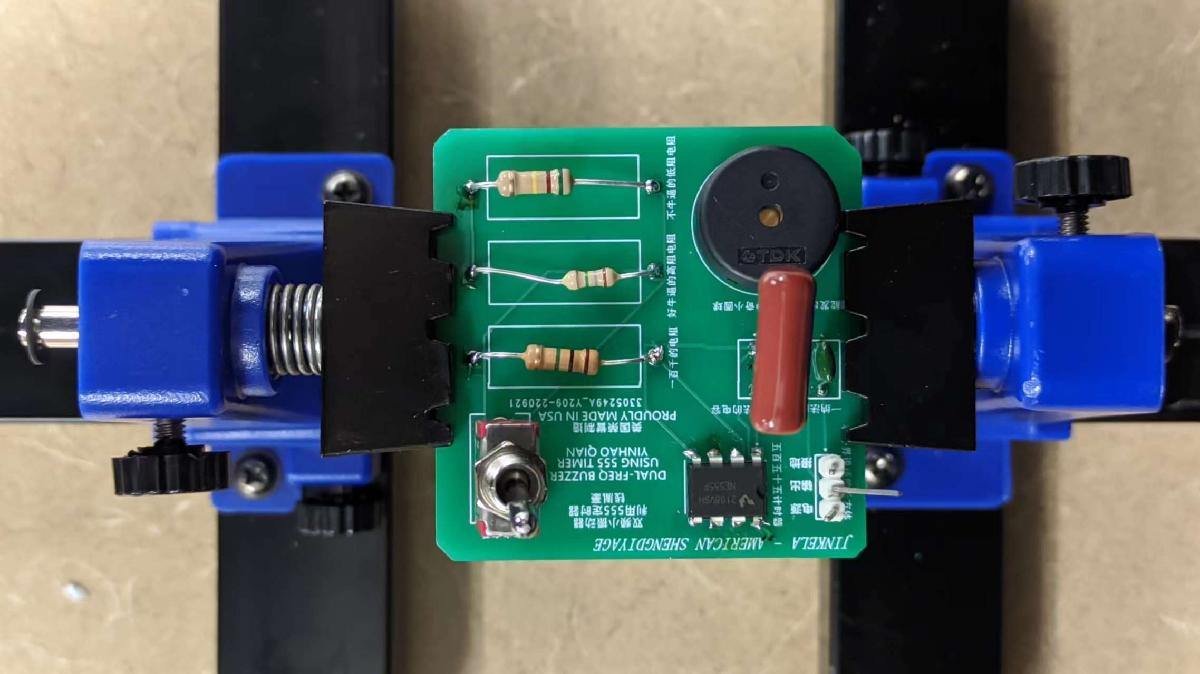
\includegraphics[width=\maxwidth{50.17561465127948em}]{image_0}
\end{flushleft}
\end{par}

\matlabheadingtwo{1.2 View from \underline{45} Deg}

\begin{par}
\begin{flushleft}
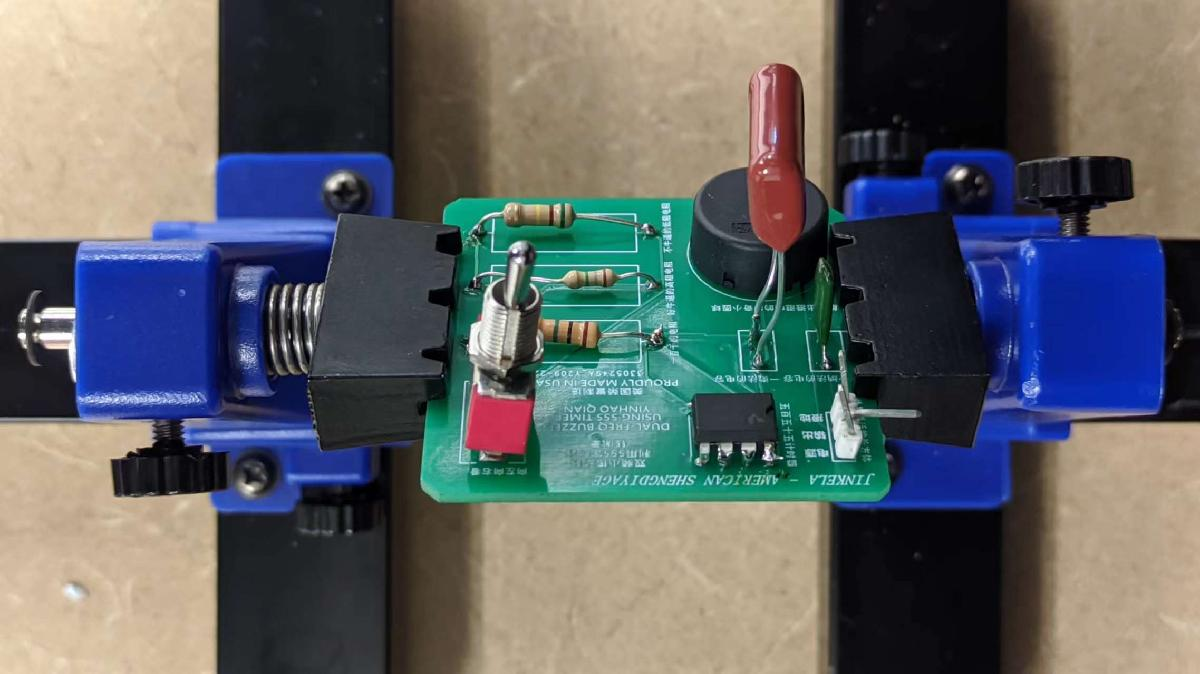
\includegraphics[width=\maxwidth{50.17561465127948em}]{image_1}
\end{flushleft}
\end{par}

\matlabheadingtwo{1.3 View from \underline{90} Deg}

\begin{par}
\begin{flushleft}
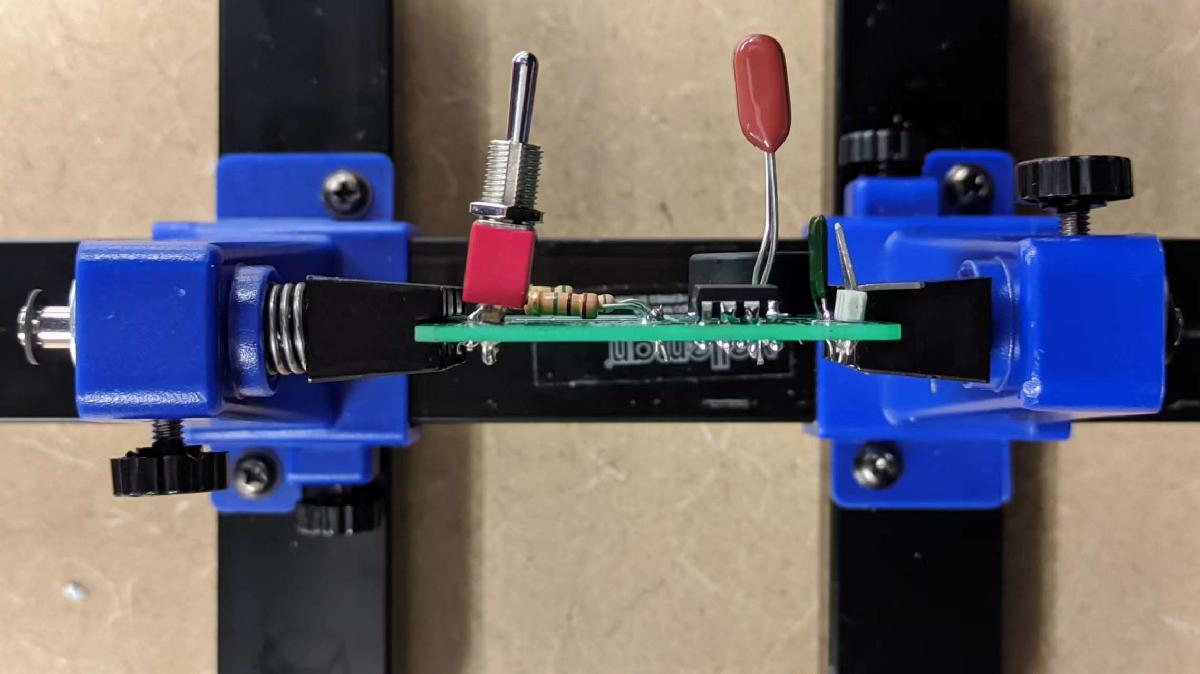
\includegraphics[width=\maxwidth{50.17561465127948em}]{image_2}
\end{flushleft}
\end{par}

\matlabheadingtwo{1.4 View from \underline{135} Deg}

\begin{par}
\begin{flushleft}
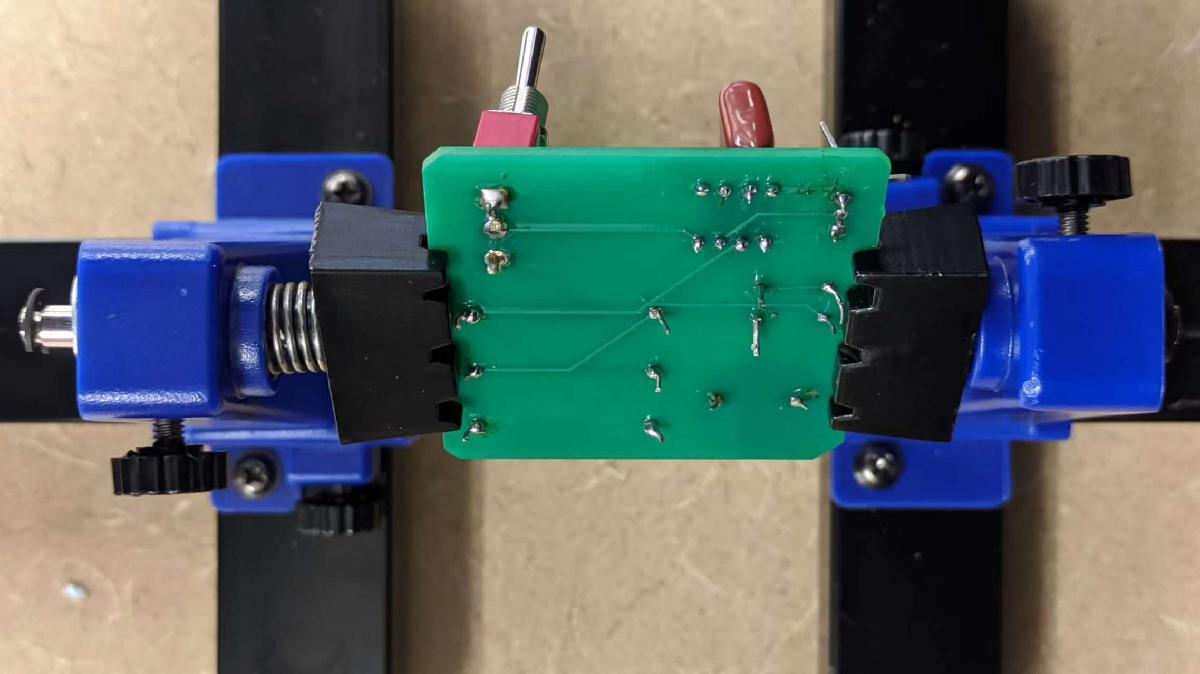
\includegraphics[width=\maxwidth{50.17561465127948em}]{image_3}
\end{flushleft}
\end{par}

\matlabheadingtwo{1.5 View from \underline{180} Deg}

\begin{par}
\begin{flushleft}
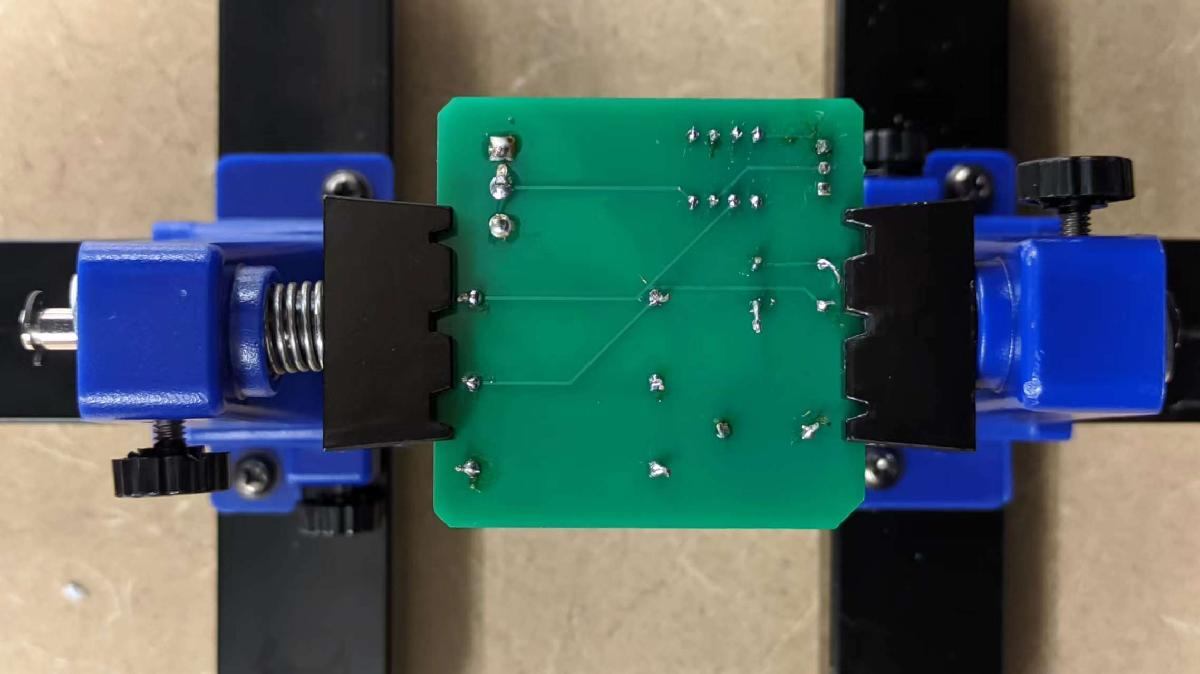
\includegraphics[width=\maxwidth{50.17561465127948em}]{image_4}
\end{flushleft}
\end{par}

\matlabheadingtwo{1.6 View from \underline{225} Deg}

\begin{par}
\begin{flushleft}
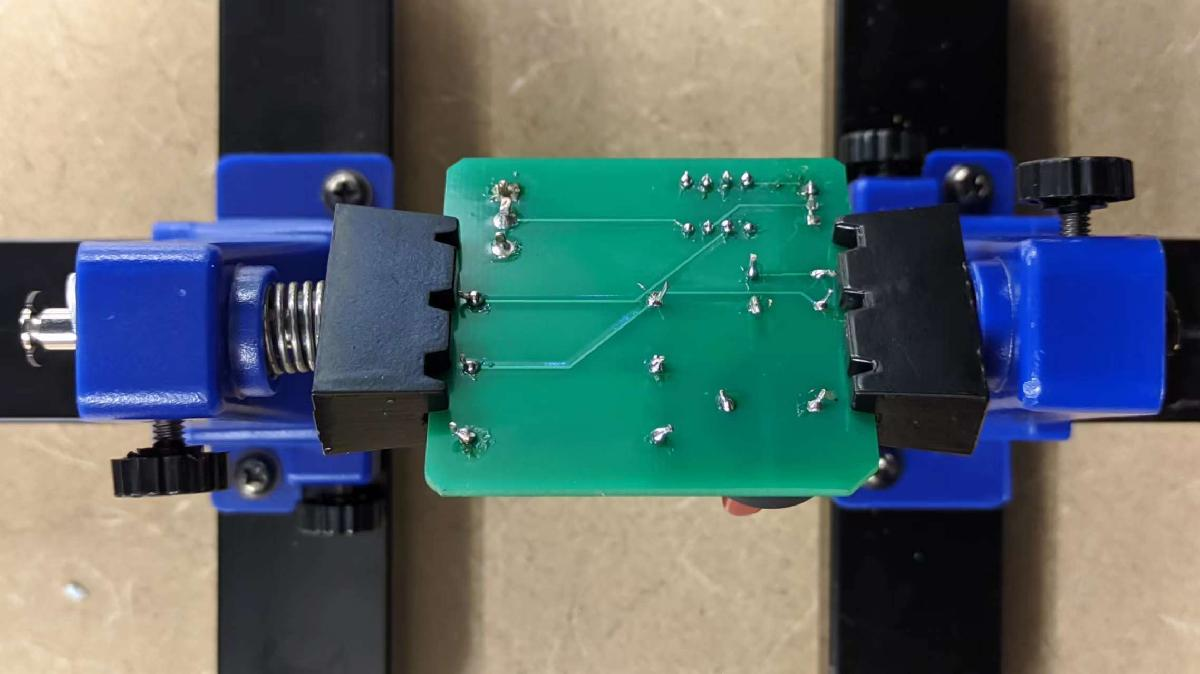
\includegraphics[width=\maxwidth{50.17561465127948em}]{image_5}
\end{flushleft}
\end{par}

\matlabheadingtwo{1.7 View from \underline{270} Deg}

\begin{par}
\begin{flushleft}
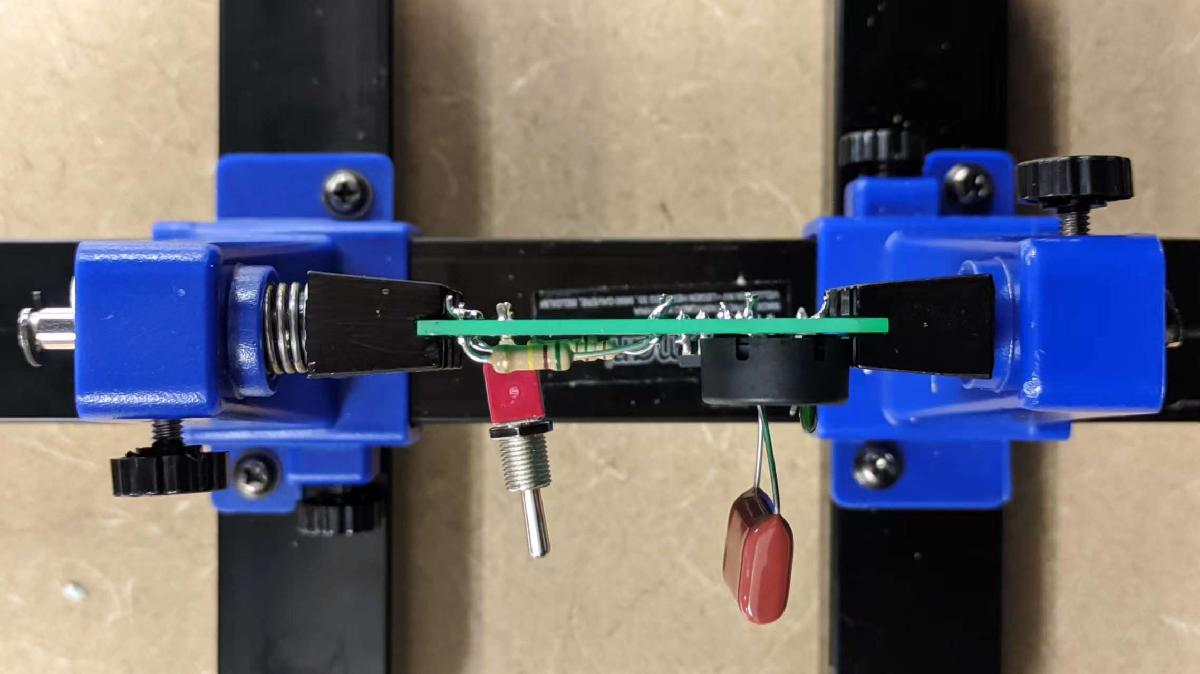
\includegraphics[width=\maxwidth{50.17561465127948em}]{image_6}
\end{flushleft}
\end{par}

\matlabheadingtwo{1.8 View from \underline{315} Deg}

\begin{par}
\begin{flushleft}
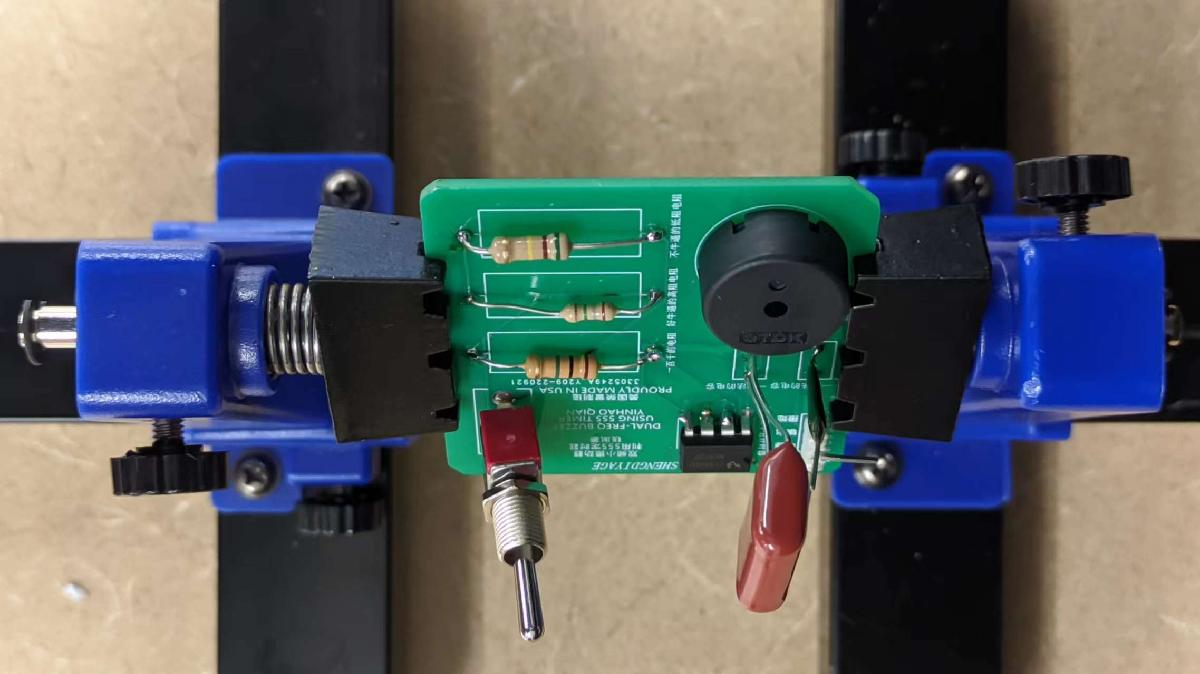
\includegraphics[width=\maxwidth{50.17561465127948em}]{image_7}
\end{flushleft}
\end{par}

\matlabheading{2 Filling Vias}

\begin{par}
\begin{flushleft}
Prior to filling the vias with solder, I have attempted to test the PCB board with all components placed, yet the PCB is not functional. This is because the connections cannot be guaranteed when the vias are not filled with conductive solder. The holes are actually a lot bigger than component pins, and angular rings would sometimes lose touch with the pins. Finally, I have used the lead-free solder that came with the practice board to fill in all the vias, making sure the solder is passed through both on the top and bottom layer. After applying the solder, the PCB is always functional. 
\end{flushleft}
\end{par}

\matlabheading{3 Evaluation Ranking}

\begin{par}
\begin{flushleft}
I personally would say I have followed almsot guidelines mentioned in class. The most important one would be reducing the board size to a square and making the components as compact as possible. Indeed, I am very satisfied with the board sizes when I first received the board. I would say one thing I can't do that is suggested during class is making the entire bottom layer as ground, since my circuit schematic requires two layers so that no crossins would exist. Overall I would say I would evaluate my board in a good rank.
\end{flushleft}
\end{par}

\end{document}
